\section{Entrega 4}


\subsection{Objetivo}

El objetivo de esta entrega es diseñar varias pruebas concretas de cada uno de los tipos y posteriormente añadirlas al proyecto. Una vez estén las pruebas terminadas, será necesario realizar un test con distintos usuarios para ver cómo funcionan y posibles mejoras que se puedan realizar.



\subsection{Iteración 1}

Durante esta iteración se van a diseñar todas las pruebas que habrá en el proyecto. Se ha elegido que haya tres pruebas de cada tipo para mostrar suficiente variedad en ellas, pero que no sean una cantidad demasiado grande para este proyecto.


\subsubsection{Pruebas de motricidad}




Para cada prueba de baile es necesario elegir una canción y tres pasos. Un paso puede ser una posición concreta de las extremidades, un movimiento concreto entre dos puntos de una extremidad, o también puede ser un momento de libertad en el que el usuario pueda moverse según le plazca al ritmo de la música. En esta prueba se busca estimular el movimiento y flexibilidad del usuario, así como su coordinación. Los momentos de libertad no solo permiten estimular estas capacidades si no que también actuan de vía de expresión para los sentimientos y estado del jugador. Es importante elegir música con la que los mayores estén familiarizados para hacer que se sientan inmersos y cómodos con la canción y el baile. Teniendo todo esto en cuenta se han elejido las siguientes tres canciones junto a sus pasos:

\begin{itemize}
    
    \item {Ejemplo 1: El chacachá del tren – El consorcio
    \begin{itemize}
        \item {Brazos arriba y abajo alternados}
        \item {Libre}
        \item {Brazos arriba y abajo alternados}
    \end{itemize}}
    
    \item {Ejemplo 2: Las flechas del amor – Karina
    \begin{itemize}
        \item {Brazo izquierdo de izquierda a derecha}
        \item {Brazo derecho de izquierda a derecha}
        \item {Libre}
    \end{itemize}}
    
    \item {Ejemplo 3: Chica ye-ye – Concha Velasco
    \begin{itemize}
        \item {Brazos arriba y abajo alternados}
        \item {Ambos brazos a la izquierda y derecha a la vez}
        \item {Libre}
    \end{itemize}}

\end{itemize}

La siguiente prueba de motricidad es la de figuras, que consiste en que el jugador adopte tres poses concretas de forma encadenada. Para que el jugador tenga tiempo de colocarse en posición, habrá cinco segundos de margen entre cada cambio de posición. Para definir un ejemplo de este tipo de prueba es necesario escoger un conjunto de tres poses corporales. Los tres ejemplos escogidos son:
	
\begin{itemize}
    	
    \item {Ejemplo 1: 
    \begin{itemize}
        \item {Ambos brazos arriba}
        \item {Brazo izquierdo abajo, derecho a la derecha}
        \item {Ambos brazos al frente}
    \end{itemize}}
    \item {Ejemplo 2:
    \begin{itemize}
        \item {Brazo derecho al frente, izquierdo arriba}
        \item {Brazo derecho en diagonal abajo, izquierdo en diagonal arriba}
        \item {Ambos brazos arriba}
    \end{itemize}}
    \item {Ejemplo 3:
    \begin{itemize}
        \item {Ambos brazos en diagonal abajo}
        \item {Ambos brazos al frente}
        \item {Ambos brazos en diagonal arriba}
    \end{itemize}}

\end{itemize}

Para la última prueba de motricidad, la de parada, el jugador tiene que repetir un movimiento de forma constante y cuando sea necesario parar en seco y mantener la posición. Con esta prueba se estimula aún más la movilidad del jugador además de su tiempo de reacción. En este caso solo es necesario definir el movimiento que el jugador seguirá, ya que el momento en el que tendrá que parar se decidirá aleatoriamente en cada prueba con un intervalo de entre 10 y 15 segundos.


\begin{itemize}
    \item {Ejemplo 1: Mover los brazos de arriba abajo al contrario (brazo derecho arriba mientras el izquierdo está abajo)}
    \item {Ejemplo 2: Trazar círculos en el frente con cada una de las manos}
    \item {Ejemplo 3: Trazar un círculo con la mano derecha mientras se sube y baja la izquierda.}
\end{itemize}


\subsubsection{Pruebas de memoria}


En las pruebas de memoria se intenta estimular la memoria a largo plazo del jugador. En la prueba de turismo se estimula la memoria mediante imágenes icónicas de diferentes ciudades y monumentos famosos a nivel mundial. La imagen se muestra en la pantalla principal del escenario del concurso y el jugador tiene que describirla, recordar su nombre, su localización y todo lo que sea capaz de recordar. Para esta prueba se han elegido las siguientes tres imágenes: 

\begin{itemize}
    \item {Ejemplo 1: Torre Eiffel, París, Francia. Figura \ref{fig:E4_torreEiffel}}
    \item {Ejemplo 2: Coliseo, Roma, Italia. Figura \ref{fig:E4_coliseo}}
    \item {Ejemplo 3: Estatua de la libertad, Nueva York, EE. UU. Figura \ref{fig:E4_estatuaLibertad}}
\end{itemize}




\begin{figure}[H]
\centering
\begin{minipage}{.3\textwidth}
  \centering
  
\includegraphics[width=.7\linewidth]{04.Desarrollo/04.Entrega4/01.Iteracion4_1/00.Figuras/01.eiffel.jpg}
  \captionof{figure}{Torre Eiffel, París, Francia.}
  \label{fig:E4_torreEiffel}
\end{minipage}%
\begin{minipage}{.3\textwidth}
  \centering
  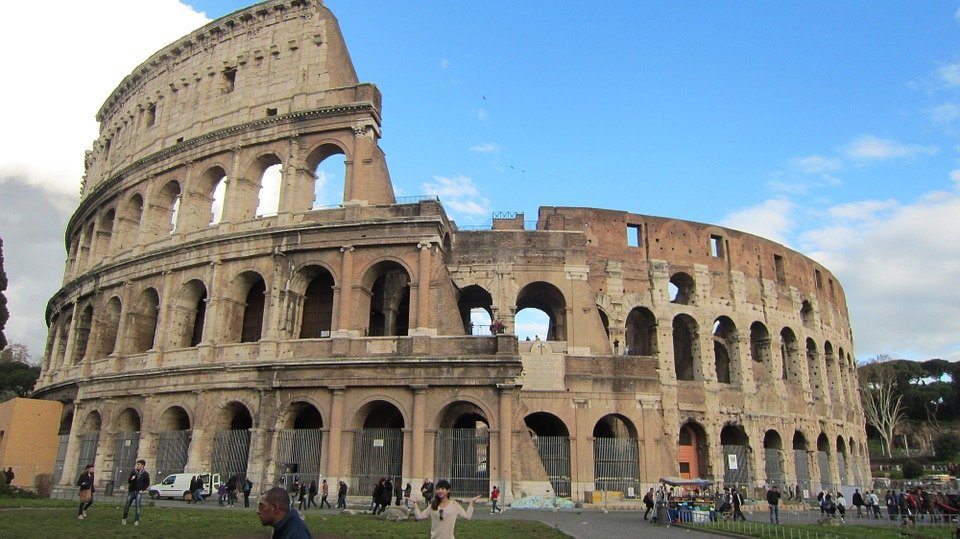
\includegraphics[width=.9\linewidth]{04.Desarrollo/04.Entrega4/01.Iteracion4_1/00.Figuras/02.coliseo.jpg}
  \captionof{figure}{Coliseo romano, Roma, Italia.}
  \label{fig:E4_coliseo}
\end{minipage}
\begin{minipage}{.3\textwidth}
  \centering
  
\includegraphics[width=.9\linewidth]{04.Desarrollo/04.Entrega4/01.Iteracion4_1/00.Figuras/03.libertad.jpg}
  \captionof{figure}{Estatua de la libertad, Nueva York, EE. UU.}
  \label{fig:E4_estatuaLibertad}
\end{minipage}
\end{figure}



La prueba de adivinar la canción utiliza el sentido del oído para despertar recuerdos y sentimientos del jugador, por esto es necesario utilizar canciones que sean reconocibles y agradables para las personas mayores cuando estén jugando. En este caso se usarán las siguientes canciones en español:

\begin{itemize}
    \item {Ejemplo 1: Dos gardenias – Antonio Machín}
    \item {Ejemplo 2: Que viva España – Manolo Escobar}
    \item {Ejemplo 3: La luna enamorada – Los Bocheros}
\end{itemize}

\subsubsection{Prueba de lenguaje}

En la prueba de situaciones se intenta que el jugador razone y hable sobre una situación concreta. Para ello se mostrará una imagen en la pantalla del escenario que representará una situación concreta. Se intenta que el jugador esté inmerso en la experiencia y pueda desarrollar sus pensamientos sobre la imagen, por lo que es importante que se traten de situaciones comunes, por las que probablemente hayan pasado y que les evoque sentimientos. Se han elegido estas imágenes:

\begin{itemize}
    \item {Ejemplo 1: Médico vendando la mano de una persona. Figura \ref{fig:E4_medico}}
    \item {Ejemplo 2: Madre preparando a su hijo para el colegio. Figura \ref{fig:E4_colegio}}
    \item {Ejemplo 3: Gente bailando en la Feria de Abril. Figura \ref{fig:E4_feria}}
\end{itemize}



\begin{figure}[H]
\centering
\begin{minipage}{.3\textwidth}
  \centering
  
\includegraphics[width=.9\linewidth]{04.Desarrollo/04.Entrega4/01.Iteracion4_1/00.Figuras/04.medico.jpg}
  \captionof{figure}{Médico vendando una mano.}
  \label{fig:E4_medico}
\end{minipage}%
\begin{minipage}{.3\textwidth}
  \centering
  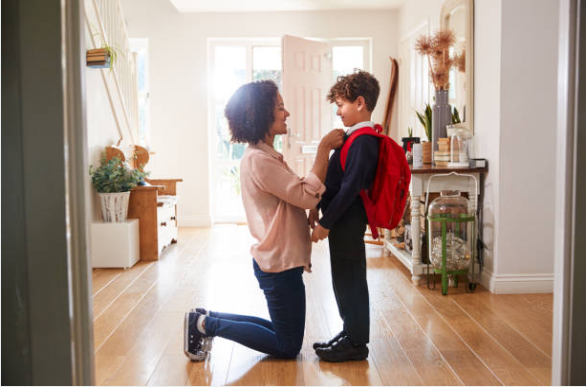
\includegraphics[width=.9\linewidth]{04.Desarrollo/04.Entrega4/01.Iteracion4_1/00.Figuras/05.colegio.png}
  \captionof{figure}{Madre preparando a su hijo para el colegio.}
  \label{fig:E4_colegio}
\end{minipage}
\begin{minipage}{.3\textwidth}
  \centering
  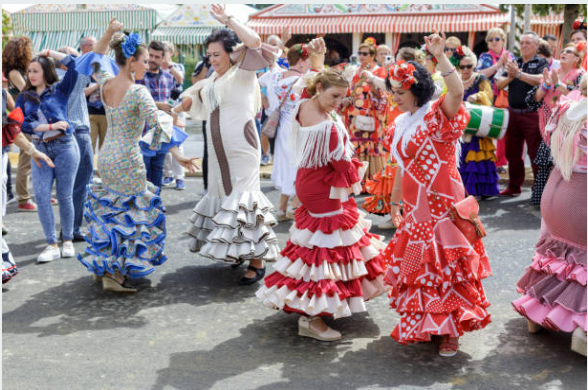
\includegraphics[width=.9\linewidth]{04.Desarrollo/04.Entrega4/01.Iteracion4_1/00.Figuras/06.feria.png}
  \captionof{figure}{Gente bailando en la feria de abril.}
  \label{fig:E4_feria}
\end{minipage}
\end{figure}


\subsubsection{Pruebas de razonamiento}


En estas pruebas se intenta activar y ejercitar el razonamiento del jugador. La prueba de agrupación de objetos intenta que el jugador descubra las dos categorías ocultas en las que se clasifican los objetos que se le muestran. Es necesario que estos objetos sean fácilmente reconocibles en forma de objeto virtual tridimensional, así como claramente distinguible la categoría a la que pertenecen cuando se presentan con el resto de los objetos. Para cada ejemplo se mostrarán cuatro objetos de dos categorías sobre la mesa del escenario:

\begin{itemize}
    \item {Ejemplo 1: 
        \begin{itemize}
            \item {Frutas: Manzana, plátano}
            \item {Ropa: Zapato, guante}
        \end{itemize}}
    \item {Ejemplo 2:
        \begin{itemize}
            \item {Transporte: Avión, coche}
            \item {Objetos de casa: Bombilla, teléfono}
        \end{itemize}}
    \item {Ejemplo 3:
        \begin{itemize}
            \item {Plantas: Árbol, flor}
            \item {Música: Guitarra, radio}
        \end{itemize}}
\end{itemize}

En la prueba de asociación de sonidos se muestran objetos sobre la mesa de la misma forma que en la prueba anterior, con la única condición de que estos objetos tienen que poder emitir un sonido característico. En este caso, se pueden usar los mismos objetos para los tres ejemplos y lo que cambiará será qué objeto produce el sonido. Para tener variedad de sonidos distinguibles, se han elegido los siguientes:

\begin{itemize}
    \item {Coche}
    \item {Pájaro}
    \item {Guitarra}
    \item {Teléfono}
\end{itemize}


\subsubsection{Pruebas de comprensión espacial}


En las pruebas de comprensión espacial se intenta evaluar la capacidad del jugador de tener una comprensión firme del espacio que lo rodea así como de los estímulos que recibe de él, principalmente mediante la audición o la visión. La prueba de siluetas presenta al usuario con tres siluetas sombreadas y debe descubrir de qué objetos se trata. Las siluetas irán en conjuntos de tres y podrán o no estar superpuestas. Para no aumentar la complejidad del proyecto, se utilizan modelos ya utilizados en otras pruebas agrupados de la siguiente forma:
	
\begin{itemize}
    \item {Ejemplo 1: Coche, teléfono, árbol.}
    \item {Ejemplo 2: Manzana, bombilla, guante.}
    \item {Ejemplo 3: Zapato, plátano, flor.}
\end{itemize}

Finalmente, la prueba de localización de sonidos consiste en colocar una fuente sonora en el espacio al rededor del usuario. El sonido será una persona hablando, ya que es un estímulo muy habitual en la vida real y las posiciones donde aparecerá se elegirán de forma aleatoria en cualquier punto del escenario fuera del campo visual del jugador.




\subsection{Iteración 2}

El objetivo de esta iteración es obtener un prototipo del juego que contenga varias pruebas de cada tipo. Se centra la atención en que las pruebas sean completamente funcionales y suficientemente variadas entre ellas.


Las pruebas implementadas en el proyecto tienen una estructura básica que funciona de igual forma para todas: da comienzo la prueba, se baja el ascensor actual, se sube el correspondiente a la prueba, se instancian todos los objetos necesarios para la prueba, se comprueba su finalización y finalmente se revierte al ascensor principal y se destruyen los objetos que no sean necesarios. Cada una de las pruebas solo se diferencia del resto en elementos concretos como: qué objetos y dónde se instancian, si tiene que reproducirse algún sonido o la mecánica concreta de la prueba. 

En cuestión de código, esto se traduce en una estructura de clases con herencia, dónde el funcionamiento concreto de cada prueba viene dado por su propia clase que a su vez hereda toda la funcionalidad general de una clase superior llamada en este caso 'Prueba'. La clase 'Prueba' es la que contiene la mayoría de la funcionalidad, como se ve en la figura \ref{fig:E4_clasePrueba}, dejando a las clases individuales únicamente como medios se preparar todo lo necesario para dicha prueba y posteriormente dar comienzo a la misma. En la figura \ref{fig:E4_cargarPrueba} se puede ver un ejemplo de como se indican los objetos que se tienen que instanciar (añadiéndolos a una lista), el ascensor correspondiente que debe aparecer y el sonido que se reproducirá.

Utilizando esta estructura de clases se potencian de forma simultánea dos aspectos del proyecto:


\begin{itemize}
    \item {Manteniendo la funcionalidad principal agrupada en una clase, se facilita la inclusión de nuevas pruebas en el futuro, siendo solo necesario crear la clase hija que prepare la prueba para su correcta ejecución.}
    \item {Tener una estructura de herencia implica que en cualquier momento una clase hija puede sobrescribir el funcionamiento de la clase original, permitiendo la implementación de pruebas completamente distintas y más complejas que las actuales.}
\end{itemize}



\begin{figure}
  \centering
    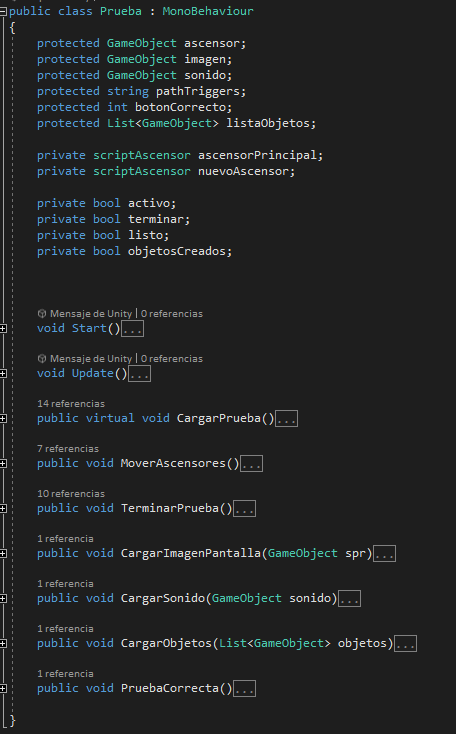
\includegraphics[width=0.5\textwidth]{04.Desarrollo/04.Entrega4/02.Iteracion4_2/00.Figuras/01.prueba.png}
    \caption{Estructura de la clase 'Prueba'.}
    \label{fig:E4_clasePrueba}
\end{figure}

\begin{figure}
  \centering
    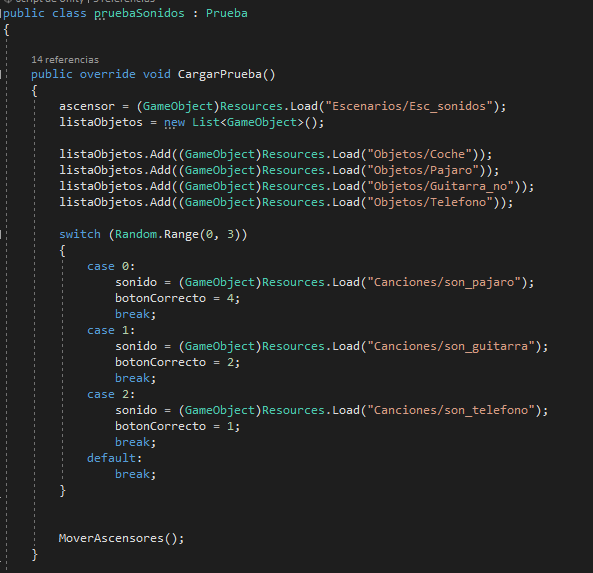
\includegraphics[width=0.7\textwidth]{04.Desarrollo/04.Entrega4/02.Iteracion4_2/00.Figuras/02.cargar_prueba.png}
    \caption{Sobrescritura del método 'CargarPrueba' para la prueba de asociación de un sonido con un objeto.}
    \label{fig:E4_cargarPrueba}
\end{figure}




\subsubsection{Pruebas de motricidad}

Para las pruebas que ejercitan la motricidad se ha utilizado la funcionalidad de los 'Triggers' creados durante el apartado \ref{E2_triggers}.

Cuando la prueba de baile da comienzo, la clase correspondiente carga la estructura de los triggers (posiciones que debe adoptar el jugador) desde un fichero JSON. También comienza a reproducir la canción requerida para la prueba correspondiente. La prueba de posiciones utiliza la misma técnica pero cargando otras estructuras diferentes y sin música, mientras que la prueba de paradas hace lo mismo pero en lugar de reproducir una canción, se prepara para reproducir un sonido que indica al jugador que tiene que detenerse.

En estas pruebas es importante la forma en la que se le transmite al usuario que posición debe adoptar. El jugador tiene que tener claro dónde tiene que colocar sus extremidades tanto vertical como horizontalmente. Un símbolo como una flecha es un icono fácilmente reconocible y con un significado muy claro si se utiliza correctamente. Teniendo en cuenta esto, un método para transmitir la información al jugador podría ser mediante flechas que aparecen delante del mismo y que indican dónde colocar las manos.

Con la idea de reflejar lo mejor posible las indicaciones al usuario, se puede utilizar una estructura que se asemeje a la propia estructura de triggers utilizada para detectar los movimientos. Mediante este paralelismo se puede mejorar la precisión y facilidad con la que el usuario capta y entiende los movimientos que tiene que hacer. De este modo, se ha creado una matriz de cuadrados con flechas que aparece frente al usuario y cambian de la misma forma que cambian los triggers (véase figura \ref{fig:E4_posiciones}).

\begin{figure}
  \centering
    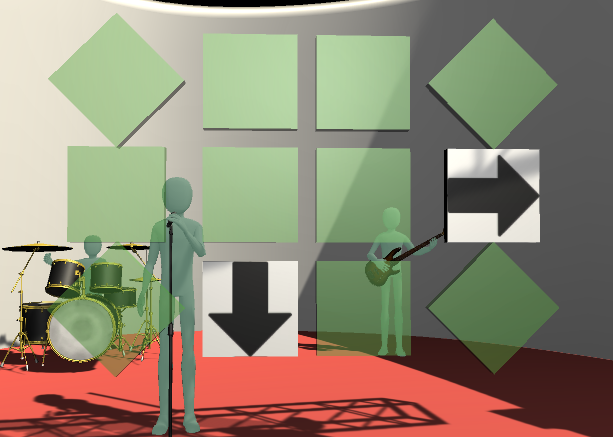
\includegraphics[width=0.7\textwidth]{04.Desarrollo/04.Entrega4/02.Iteracion4_2/00.Figuras/03.posiciones.png}
    \caption{Matriz de señales que indican al usuario dónde colocar sus manos.}
    \label{fig:E4_posiciones}
\end{figure}


\subsubsection{Pruebas de memoria}

Las pruebas de memoria se basan en presentar una imagen o canción al jugador para hacerle recordar información sobre ellas o revivir experiencias personales que tenga asociadas con ellas. Para la reproducción de las canciones se utiliza un objeto nativo de Unity llamado Audio Source. Es un objeto que permite reproducir un clip de audio dentro de la escena del juego. Por lo tanto, solo es necesario indicar qué clip de audio sonará durante cada prueba como se muestra en la figura \ref{fig:E2_audioSource}. Esta misma técnica es la que se utiliza para todas las pruebas que necesiten reproducir algún sonido.

\begin{figure}
  \centering
    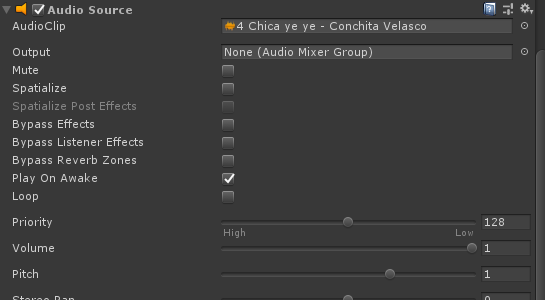
\includegraphics[width=0.7\textwidth]{04.Desarrollo/04.Entrega4/02.Iteracion4_2/00.Figuras/04.audio_source.png}
    \caption{Audio Source de Unity mostrando el clip actual que reproduce, así como otros de sus parámetros.}
    \label{fig:E4_audioSource}
\end{figure}


Para las pruebas en las que se presenta al jugador una imagen, se utiliza una primitiva de Unity que permite crear planos bidimensionales dentro de una escena 3D. Utilizando la pantalla gigante que forma parte del escenario se coloca sobre ella un plano en el que posteriormente se puede colocar como textura del mismo cualquier imagen. De esta forma, solo es necesario activar y desactivar el plano junto con su textura correspondiente. En la imagen \ref{fig:E4_imagen} se representa un objeto de tipo plano, que muestra una imagen del coliseo romano.

\begin{figure}
  \centering
    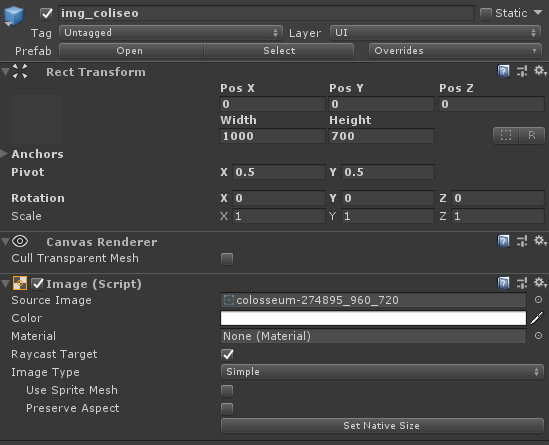
\includegraphics[width=0.7\textwidth]{04.Desarrollo/04.Entrega4/02.Iteracion4_2/00.Figuras/05.imagen.png}
    \caption{Parámetros de un objeto plano de Unity mostrando una imagen del coliseo romano.}
    \label{fig:E4_imagen}
\end{figure}


\subsubsection{Prueba de lenguaje}

En esta prueba se presenta al jugador una imagen en la que aparece una situación cotidiana, que puede haber vivido, con el objetivo de que hable y haga comentarios sobre ella. Para esto solo en necesario mostrar una imagen en la pantalla gigante del escenario, siguiendo la misma técnica usada en la prueba anterior.

\subsubsection{Pruebas de razonamiento}


Para las pruebas de razonamiento se utiliza una mesa frente al jugador en la que aparecen varios objetos con los que debe interactuar para superar el reto. En la prueba de agrupación de objetos (véase figura \ref{fig:E4_asociacion}), además es necesario crear dos zonas donde categorizar los objetos. Estas zonas pertenecen a la propia mesa y siempre son las mismas. Para cada ejemplo de esta prueba solo es necesario cambiar los objetos que se instancian. Para asegurar que todos los objetos aparecen en el lugar adecuado, se han creado cuatro objetos vacíos, asociados a la mesa, que sirven únicamente como punto de referencia. A la hora de instanciar los objetos, se buscan estas referencias y se genera un objeto en la posición de cada una. 

En la figura \ref{fig:E4_mesa} se puede ver la estructura de objeto para la mesa, que está compuesta por dos piezas (suelo y mesa), así como dos conjuntos de objetos, el primero de ellos, las 'SpawnZone' que marcan los puntos donde aparecerán los objetos; y el segundo son las plataformas donde deben colocarse los objetos para considerarse clasificados.



\begin{figure}
  \centering
    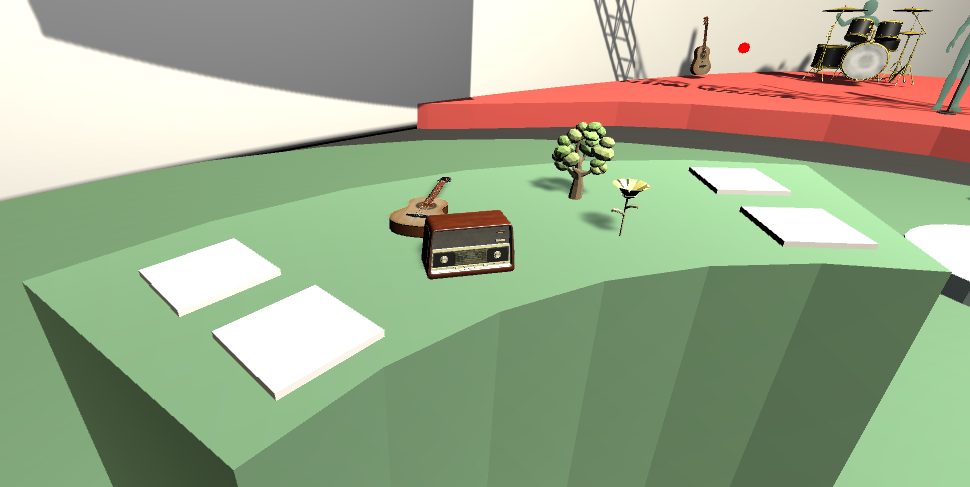
\includegraphics[width=0.7\textwidth]{04.Desarrollo/04.Entrega4/02.Iteracion4_2/00.Figuras/06.asociacion.png}
    \caption{Ejemplo de prueba de agrupación de objetos.}
    \label{fig:E4_asociacion}
\end{figure}


\begin{figure}
  \centering
    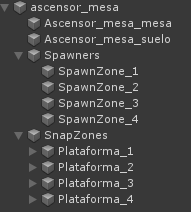
\includegraphics[width=0.4\textwidth]{04.Desarrollo/04.Entrega4/02.Iteracion4_2/00.Figuras/07.mesa.png}
    \caption{Estructura de objeto para la mesa.}
    \label{fig:E4_mesa}
\end{figure}



En la prueba de asociación de sonidos, en lugar de necesitar zonas para clasificar los objetos es necesario crear cuatro botones, uno correspondiente a cada objeto (véase figura \ref{fig:E4_sonidos}). Cada uno de estos botones puede ejecutar un método del código cuando se pulsa. Esto es lo que se utiliza para detectar la respuesta correcta, ya que en tiempo de ejecución, cuando se crean los objetos, automáticamente se asigna que el botón adecuado llame al método para dar la prueba por correcta, como se puede ver en la figura \ref{fig:E4_botonCorrecto}.


\begin{figure}
  \centering
    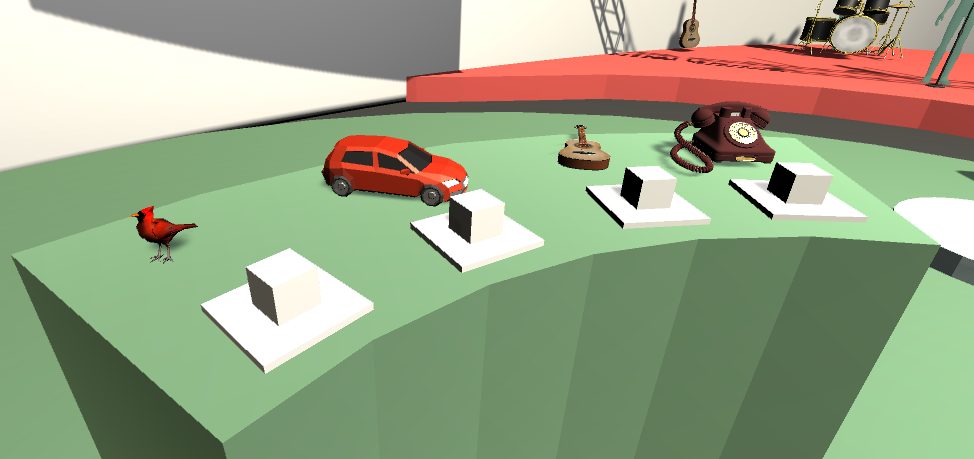
\includegraphics[width=0.7\textwidth]{04.Desarrollo/04.Entrega4/02.Iteracion4_2/00.Figuras/08.sonidos.png}
    \caption{Ejemplo de prueba de asociación de sonidos.}
    \label{fig:E4_sonidos}
\end{figure}

\begin{figure}
  \centering
    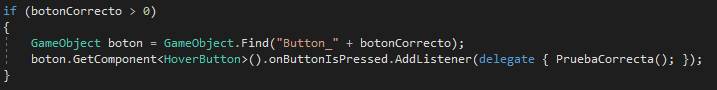
\includegraphics[width=0.9\textwidth]{04.Desarrollo/04.Entrega4/02.Iteracion4_2/00.Figuras/09.boton_correcto.png}
    \caption{Código que asigna la llamada al método para terminar la prueba de forma correcta al botón adecuado.}
    \label{fig:E4_botonCorrecto}
\end{figure}




\subsubsection{Pruebas de comprensión espacial}

Para la prueba de localización de sonidos se usa la misma técnica para la reproducción de audio usada en el resto de pruebas, pero con ligeras diferencias. En el objeto Audio Source que se encarga de reproducir el sonido, es necesario activar el parámetro 'Spatialize' (ya visto en la figura \ref{fig:E4_audioSource}), ya que es el que permite oír el sonido en 3D. La otra diferencia es que la fuente de sonido puede aparecer en cualquier punto del espacio al rededor del jugador salvo a su frente. Para esto último se generan en tiempo de ejecución tres valores en ciertos intervalos controlados para acotar el espacio posible.





\subsection{Iteración 3}


En esta última iteración se busca que un usuario real realice las distintas pruebas para poder evaluarlas, encontrar posibles problemas y solucionarlos. Para ello se cuenta con una persona joven, con conocimientos tecnológicos básicos. Esta persona ha repetido varias veces cada una de las pruebas creadas en este proyecto y de su experiencia se pueden sacar las siguientes conclusiones sobre las pruebas:


\begin{itemize}
    \item {Durante las pruebas de baile y figuras, en las que el jugador debe colocar sus manos en posiciones determinadas, es necesario reevaluar el tiempo entre cada pose, ya que a veces este tiempo es demasiado largo y en otras ocasiones, dependiendo de la pose, resulta un poco corto.}
    \item {En la prueba de asociación de objetos en necesario ajustar la posición de cada objeto y zona para que el jugador llegue cómodamente a todas ellas. Además, actualmente, no hay forma de recuperar un objeto en caso de que cayera a un lugar inaccesible.}
    \item{La elección de canciones para las pruebas de baile y adivinar la canción, parece ser muy buena.}
    \item{Los sonidos usados en la prueba de asociación de sonidos son claros y fácilmente distinguibles, lo cual es bueno.}
    \item{La posición aleatoria de la fuente de sonido en la prueba donde hay que localizarla puede ser problemática. Hay zonas en las que es muy difícil distinguir la procedencia del sonido.}
\end{itemize}






\subsection{Conclusiones de la entrega}

A pesar de tener las mecánicas básicas implementadas en la entrega 2, esta entrega ha sido la más compleja hasta ahora y ha requerido el mayor tiempo. Especialmente, crear la estructura de clases y toda la funcionalidad básica que trabaje en conjunto y adecuadamente para los distintos tipos de pruebas. 

Ha sido particularmente importante poder encontrar canciones e imágenes que el público objetivo del juego (personas mayores) pueda reconocer sin problema y que además, las canciones sean capaces de animarlos o despertar algún sentimiento o memoria.

Finalmente se han encontrado algunos problemas, como que es necesario ajustar el tiempo entre cada posición en las pruebas de motricidad. Posiblemente se necesite más tiempo del que se deja en principio, pero lo ideal sería poder variar este tiempo de forma dinámica para adaptarse a cada jugador. La prueba de localización de sonidos también tiene un problema dependiendo de la posición en la que aparezca la fuente de sonido. Por esto, es mejor cambiar la forma en la que se coloca dicha fuente: en lugar de utilizar una posición aleatoria se pueden definir una serie de posiciones que se consideren adecuadas, de las cuales se elegirá entre una de ellas al comenzar la prueba, asegurando así que la localización será siempre adecuada.



